\section{Kurzfristfinanzierung und Working Capital Management}

\textbf{Motivation}: Wahrung des finanziellen Gleichgewichts erfordert
\begin{itemize}
	\item Detaillierte Planung zukünftiger Ein- und Auszahlungen, um den Kapitalbedarf rechtzeitig zu identifizieren
	\item Bestimmung der vorzuhaltenden Liquiditätsreserven (Cash Management) und Messung von Liquidität
	\item Verhindern von Liquiditätsengpässen (Working Capital Management, Kurzfristfinanzierung)
\end{itemize}
\bigskip
\textbf{Was ist Cash bzw. Liquidität?}
\begin{itemize}
	\item \textbf{Zahlungsmittel}: Kassenbestand, Kredite, Schecks
	\item \textbf{Zahlungsmitteläquivalente}: Kurzfristige, sehr liquide Geldanlagen wie z.B. Schatzbriefe oder Geldmarktfonds $\rightarrow$ leicht veräußerbar, geringe Wertänderungsrisiken
\end{itemize}
\bigskip
\textbf{Motive und Determinanten der Liquiditätshaltung}:
\begin{itemize}
	\item \textbf{Motive}: Vorsichtsmotiv, strategische Motive, Transaktionsmotive
	\item \textbf{Determinanten}:
	\begin{itemize}
		\item Volatilität der Cash Zu- und Abflüsse $[+]$
		\item Kapitalmarktzugang und Kreditfähigkeit des Unternehmens $[-]$
		\item Effizienz des Cash-Flow bzw. Working Capital Management $[-]$
	\end{itemize}
\end{itemize}
\bigskip
\textbf{Kosten der Liquiditätshaltung}: $\rightarrow$ \textbf{Opportunitätskosten}, z.B. Entgangene Zinserträge, Steuernachteile

\textbf{Kosten unzureichender Liquiditätsreserven}: $\rightarrow$ \textbf{Transaktionskosten} für Verkauf von Vermögensgegenständen sowie Kosten für kurzfristige Kreditaufnahme 

\begin{center}
	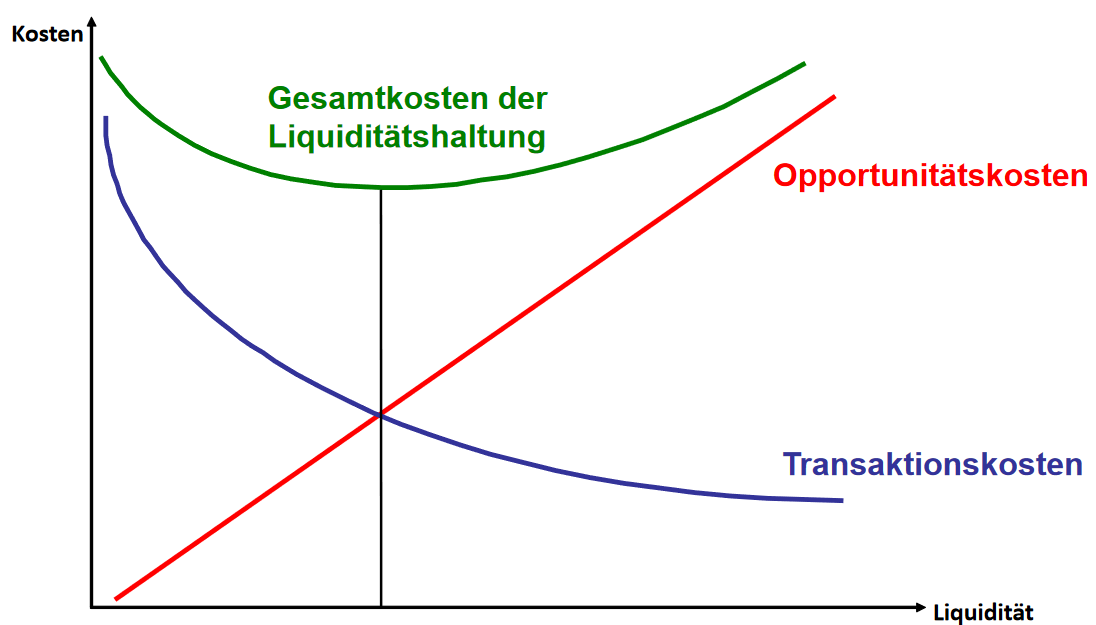
\includegraphics[width=0.5\textwidth]{images/cash-level.png}
\end{center}
\bigskip
\textbf{Liquiditätsgrade}: Möglichkeit, Vermögensgegenstände in Geld umzuwandeln $\rightarrow$ signalisieren kurzfristigen Kreditgebern Zahlungssicherheit
\begin{itemize}
	\item \textbf{Cash Ratio} $=\cfrac{\text{liquide Mittel}}{\text{kurzfristige Verbindlichkeiten}}$ 
	
	gibt an, inwieweit ein Unternehmen seine Zahlungsverpflichtungen durch seine liquiden Mittel erfüllen kann
	
	\item \textbf{Acid Test Ratio}$=\cfrac{\text{liquide Mittel}+\text{kurzfristige Forderungen}}{\text{kurzfristige Verbindlichkeiten}}$
	
	$\text{ATR} < 1$: Teil der kurzfristigen Verbindlichkeiten wird nicht durch kurzfristig zur Verfügung stehendes Vermögen gedeckt
	
	\item \textbf{Current Ratio}$=\cfrac{\text{Umlaufvermögen}}{\text{kurzfristige Verbindlichkeiten}}$
	
	ATR um Vorräte erweitert, Wert $>$ 1 als Untergrenze, sonst muss Deckung kurzfristiger Verbindlichkeiten durch den Verkauf von Anlagevermögen erfolgen
\end{itemize}
\bigskip
\textbf{Working Capital Management}: Aus Kapitalbindung im Produktionsprozess resultiert ein Kapitalbedarf $\rightarrow$ Kapitalbedarf managen, um Gesamtkosten zu minimieren
\begin{itemize}
	\item \textbf{Working Capital}: Vermögensteile, die sich innerhalb eines Produktionszyklus in liquide Mittel zurückverwandeln
	\item \textbf{Net Working Capital} ist das Nettoumlaufvermögen:
	
	$\text{NWC}=(\text{Umlaufvermögen}-\text{liquide Mittel}-\text{kurzfr. finanz. Vermögenswerte})-(\text{kurzfr. Verbindlichkeiten}-\text{kurzfr. Finanzverbindlichkeiten})$
	
	\item \textbf{Hauptbestandteile des Net Working Capital}:
	\begin{center}
		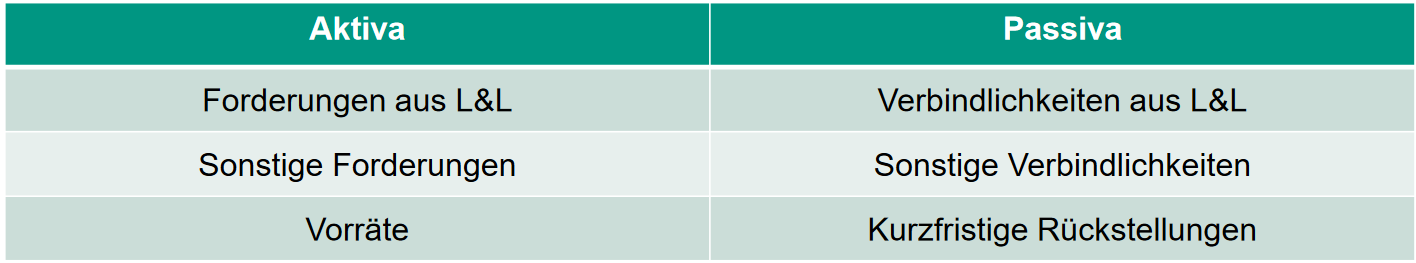
\includegraphics[width=0.75\textwidth]{images/nwc.png}
	\end{center}
\end{itemize}

\textbf{Cash Conversion Cycle (CCC)}:
\begin{center}
	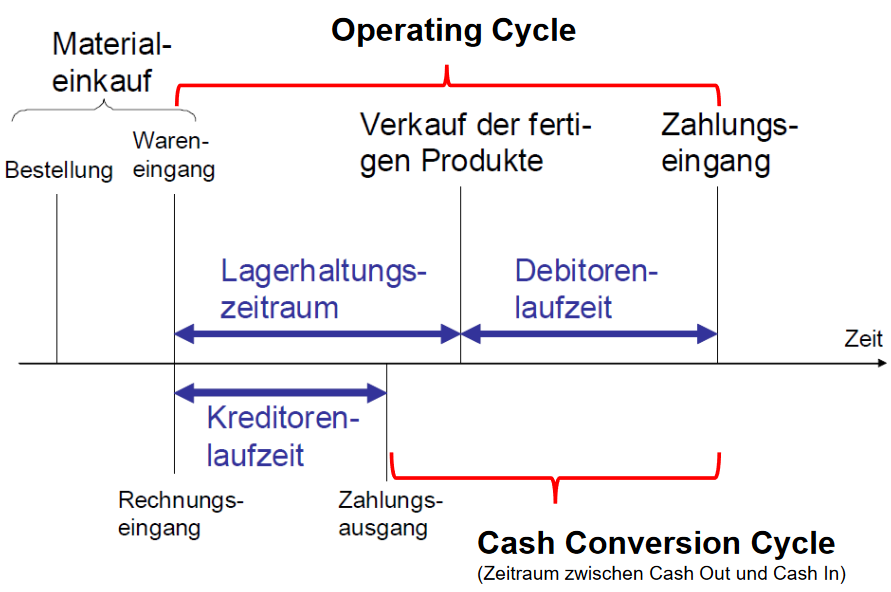
\includegraphics[width=0.5\textwidth]{images/ccc.png}
\end{center}
\begin{itemize}
	\item Länge des CCC bestimmt den Bedarf an Net Working Capital und damit auch Finanzierungsbedarf und Finanzierungskosten
	\item \textbf{Ziel}: \textbf{Geldumschlagsdauer} (Kapitalbindung) gering halten
	
	$\text{Geldumschlagsdauer}=\text{Durchschnittliche Lagerdauer } + \text{ Durchnittliche Inkassoperiode} \newline \text{(Debitorenlaufzeit)}-\text{Lieferantenzahlungsziel}$
	
	mit $\text{Durchschnittliche Lagedauer}=\cfrac{\text{Durchschn. Lagerbestand} \cdot 360 \text{ Tage}}{\text{Jahresverbrauch}}$
\end{itemize}
\bigskip
\textbf{Ziel des Working Capital Management}: Reduzierung des Net Working Capital und somit Reduktion der Finanzierungskosten

\textbf{Maßnahmen des Working Capital Management}:
\begin{enumerate}
	\item \textbf{Management der Vorratshaltung}: z.B. Standardisierung von Bauteilen, Beschaffungslagerhaltungsoptimierung
	\item \textbf{Forderungsmanagement}: 
	\begin{itemize}
		\item \textbf{Handelskredite}: Unternehmen nehmen Kredite von Lieferanten auf und gewähren ihren Kunden Kredite (abhängig von Ausfallwahrscheinlichkeit und Höhe des Kredits des Kunden, Verfügbarkeit von Sicherheiten)
		\item \textbf{Factoring}: Verkauf von Forderungen an eine Spezialbank (Factor), Unternehmen und Factor einigen sich auf Konditionen
		\begin{center}
			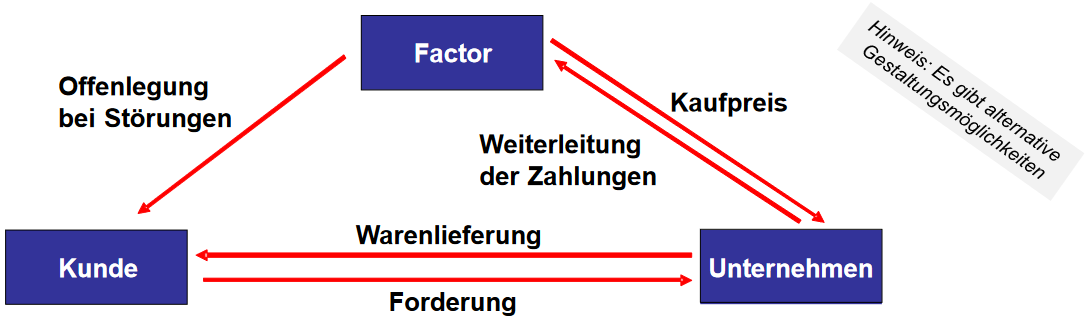
\includegraphics[width=0.6\textwidth]{images/factoring.png}
		\end{center}
		\pagebreak
		
		\item \textbf{Supply Chain Finance/Reverse Factoring}: 
		\begin{center}
			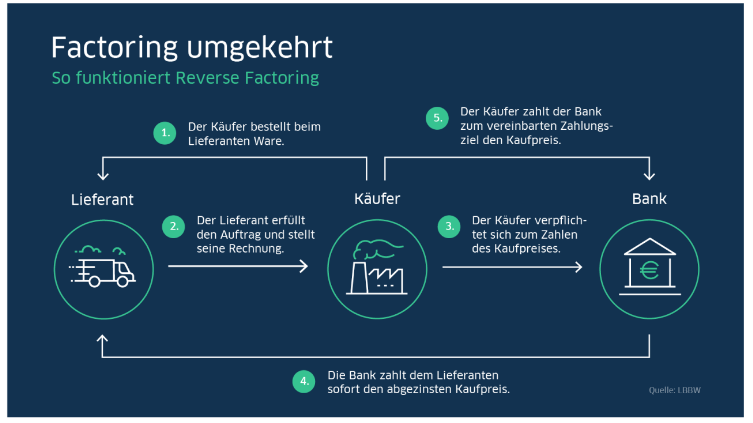
\includegraphics[width=0.6\textwidth]{images/reverse-factoring.png}
		\end{center}
	\end{itemize}
	\item \textbf{Management der Verbindlichkeiten}
\end{enumerate}
\bigskip
\textbf{Politiken der Kurzfristfinanzierung}:
\begin{itemize}
	\item Deckung langfristiger Investitionen durch Langfristfinanzierung
	\item Deckung kurzfristiger Investitionen durch Kurzfristfinanzierung
	\item Finanzierung von langfr. Betriebskapital mit kurzfristigem Kapital: \textbf{aggressive Finanzierungspolitik} $\rightarrow$ führt zu hohem Finanzierungsbedarf $\rightarrow$ Opportunitätskosten
	\item Finanzierung von kurzfr. Betriebskapital mit langfristigem Kapital: \textbf{konservative Finanzierungspolitik} $\rightarrow$ führt zu niedrigerem Finanzierungsbedarf $\rightarrow$ potentieller Verlust von Kunden, Finanzierungsengpässe
\end{itemize}

